\documentclass{beamer}

\usepackage{tikz}
\usepackage{graphicx}
\usepackage[table, x11names]{xcolor}
\usepackage{xstring}
\usepackage{etoolbox}
\usepackage{tabularx}
\usepackage[export]{adjustbox}

\newcommand{\Date}{}

\newcommand{\setDate}[1]{\renewcommand{\Date}{#1}}

\useinnertheme{default}
\useoutertheme{default}
\usecolortheme{default}

\definecolor{aziendaPrimary}{RGB}{84, 150, 104}
\setbeamercolor{structure}{fg=aziendaPrimary}
\setbeamercolor{frametitle}{bg=aziendaPrimary!10,fg=aziendaPrimary}

% rimuovere i simboli di navigazione
\setbeamertemplate{navigation symbols}{}

% pagina iniziale
\setbeamertemplate{title page}{
  \vspace{2em}
  \begin{center}
    \begin{minipage}{0.3\textwidth}
      \centering
      
\includegraphics[height=2.1cm, left]{./logounipd.png}
    \end{minipage}
    \begin{minipage}{0.3\textwidth}
      \centering
      
\includegraphics[height=2.5cm, center]{../logo-crop.pdf}
    \end{minipage}
    \begin{minipage}{0.3\textwidth}
      \centering
      
\includegraphics[height=2cm, right]{./logoview4life.png}
    \end{minipage}
  \end{center}
  \begin{center}
      {\usebeamerfont{title}\color{black}\textbf{\inserttitle}\par}
    \vspace{0.5em}
    {\usebeamerfont{date}\insertauthor\par}
    {\usebeamerfont{date}\Date\par}
  \end{center}
}

% footer
\setbeamertemplate{footline}{
  \vspace{2ex}
  \hbox{
    \begin{minipage}[t]{0.40\paperwidth}
      \hspace*{0.5em}
      \raggedright\usebeamerfont{footline}{Progetto View4Life}
    \end{minipage}%
    \begin{minipage}[t]{0.20\paperwidth}
      \centering\usebeamerfont{footline}Slide \insertframenumber{} di \inserttotalframenumber
    \end{minipage}%
    \begin{minipage}[t]{0.40\paperwidth}
      \hfill
      \insertshortauthor
      \hspace*{0.8em}
      \raisebox{-0.25\height}{
\includegraphics[width=0.7cm]{../logo-crop.pdf}}
      \hspace*{1.3em}
    \end{minipage}
  }
  \vspace{0.8ex}
}

\usepackage[absolute,overlay]{textpos}

\title{Progetto View4Life del corso \\ di Ingegneria del Software}
\author{Presentazione del \textit{Minimum Viable Product}}
\setDate{8/04/2026}

\begin{document}

{
\setbeamertemplate{footline}{}
\begin{frame}
  \titlepage
\end{frame}
}

\begin{frame}{L'obiettivo del progetto}
  % \begin{textblock*}{2cm}(10.5cm,0.5cm)
  %   \includegraphics[width=2cm]{immagine}
  % \end{textblock*}
  Sviluppare un applicativo \textit{web} per permettere la gestione delle residenze protette da parte del personale sanitario
  e dell'amministratore, tramite l'uso dei dispositivi \textit{IoT} della gamma \textit{View Wireless}. \\
  In particolare, l'applicativo deve:
  \begin{itemize}
    \item Visualizzare le informazioni dei vari \textbf{dispositivi};
    \item gestire gli stati degli \textbf{allarmi}, che verranno presi in carico dal personale sanitario;
    \item visualizzare le \textbf{\textit{analytics}} relative alla piattaforma e agli impianti, con relativi suggerimenti
          per il \textbf{risparmio energetico};
    \item visualizzare una \textbf{\textit{dashboard}} contenente le informazioni principali (stato dispositivi, allarmi attivi, ...).
  \end{itemize}
\end{frame}

\begin{frame}{Avanzamento fino ad oggi}
  \centering
  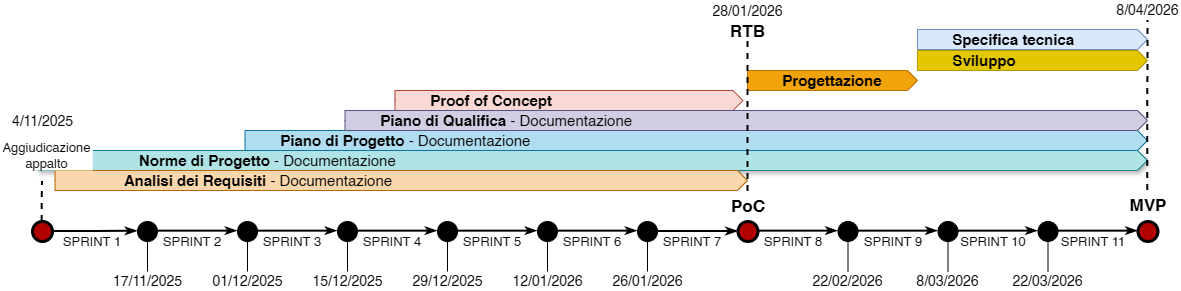
\includegraphics[
    width=\textwidth,
    height=\textheight,
    keepaspectratio
  ]{stato_avanzamento.drawio.png}
\end{frame}

\begin{frame}{Autenticazione: funzionalità (1/3)}

\end{frame}

\begin{frame}{Autenticazione: flusso(2/3)}
  
\end{frame}

\begin{frame}{Autenticazione: interfaccia(3/3)}
  
\end{frame}

\begin{frame}{Dashboard: funzionalità (1/2)}
La dashboard è la schermata principale dell'applicativo e permette di ottenere una panoramica dello stato
dell'impianto.\\
Prevede la possibilità di:
\begin{itemize}
\item Visualizzare la lista degli allarmi con priorità maggiore e di prenderli in carico;
\item consultare i consumi energetici e le statistiche sugli allarmi;
\item visualizzare una panoramica strutturale dell'appartamento e i dispositivi contenuti.
\end{itemize}
\end{frame}

\begin{frame}{Dashboard: interfaccia(2/2)}
  \centering
  
\includegraphics[
    width=\textwidth,
    height=\textheight,
    keepaspectratio
  ]{dashboard.png}
\end{frame}

\begin{frame}{Gestione Allarmi: funzionalità (1/3)}

\end{frame}

\begin{frame}{Gestione Allarmi: flusso (2/3)}
  \centering
  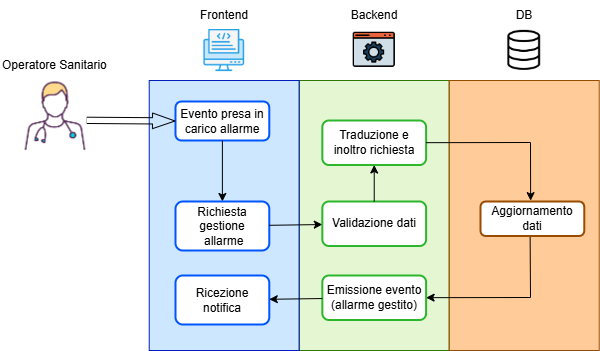
\includegraphics[
    width=\textwidth,
    height=\textheight,
    keepaspectratio
  ]{gestione-allarmi-flusso.png}
\end{frame}

\begin{frame}{Gestione Allarmi: interfaccia (3/3)}
  \centering
  
\includegraphics[
    width=\textwidth,
    height=\textheight,
    keepaspectratio
  ]{gestione-allarmi.png}
\end{frame}

\begin{frame}{Configurazione Allarmi: funzionalità (1/3)}
\end{frame}

\begin{frame}{Configurazione Allarmi: interfaccia (2/3)}
  \centering
  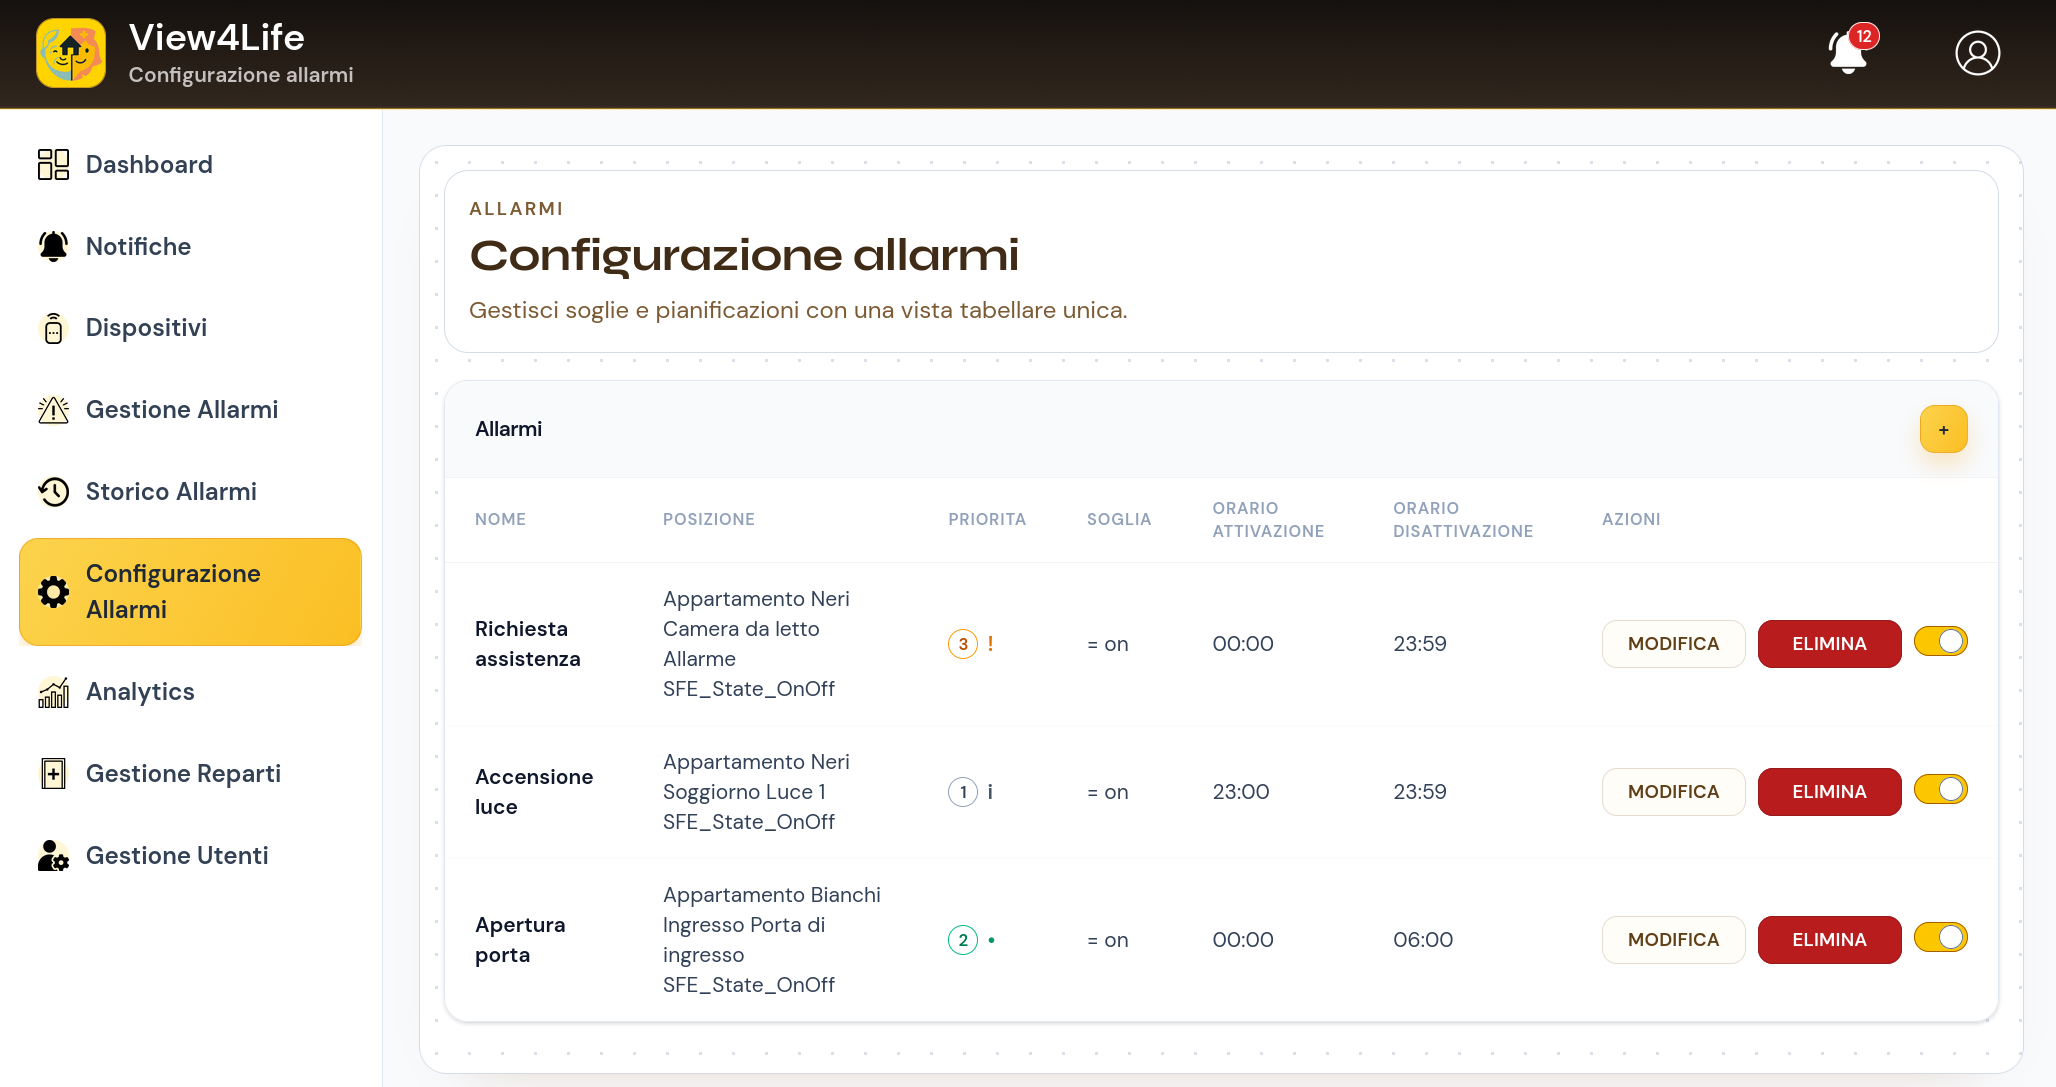
\includegraphics[
    width=\textwidth,
    height=\textheight,
    keepaspectratio
  ]{configurazione-allarmi.png}
\end{frame}

\begin{frame}{Configurazione Allarmi: interfaccia (3/3)}
  \centering
  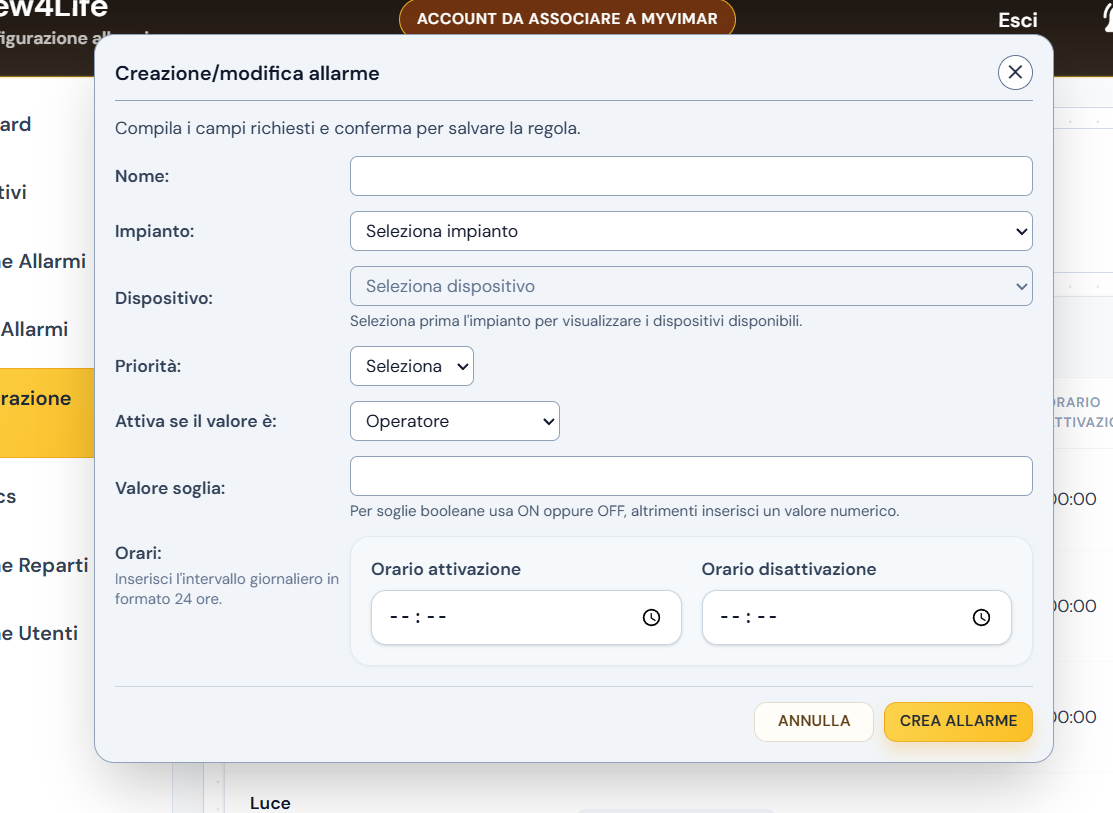
\includegraphics[
    width=\textwidth,
    height=\textheight,
    keepaspectratio
  ]{configurazione-allarme-1.png}
\end{frame}

\begin{frame}{Analytics: funzionalità (1/3)}

\end{frame}

\begin{frame}{Analytics: flusso (2/3)}
  \centering
  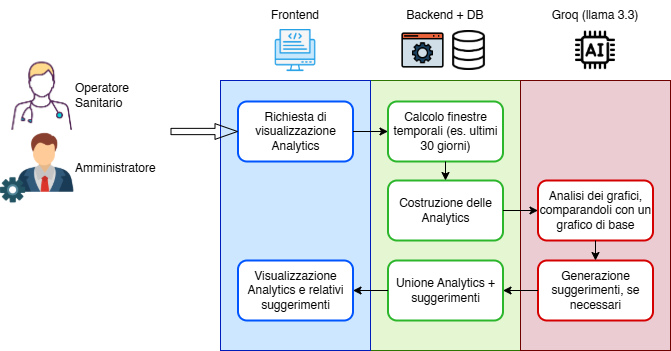
\includegraphics[
    width=\textwidth,
    height=\textheight,
    keepaspectratio
  ]{analytics-flusso.png}
\end{frame}

\begin{frame}{Analytics: interfaccia (3/3)}
  \centering
  
\includegraphics[
    width=\textwidth,
    height=\textheight,
    keepaspectratio
  ]{analytics.png}
\end{frame}

\begin{frame}{Altre funzionalità amministratore}
La figura dell'amministratore ha inoltre accesso alle seguenti funzionalità:
\begin{itemize}
  \item Gestione Reparti: permette di amministrare le relazioni di appartenenza appartamento-reparto e operatore sanitario-reparto.
  \item Gestione Utenti: permette la creazione e l'eliminazione di utenti.
\end{itemize}
\end{frame}

\begin{frame}{Modello architetturale(1/2)}
 \centering
  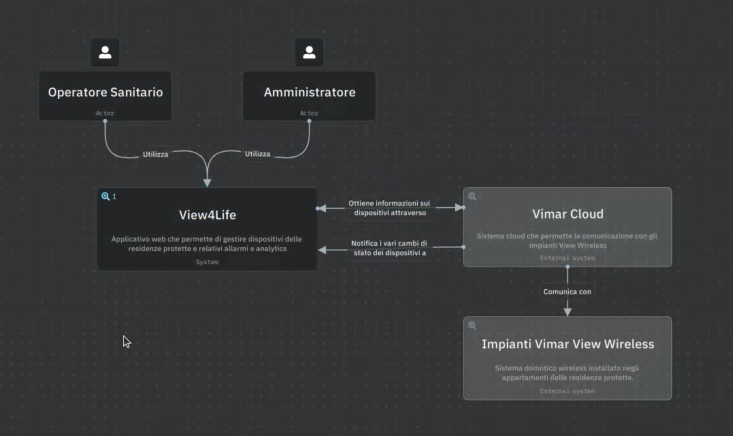
\includegraphics[
    width=\textwidth,
    height=0.8\textheight,
    keepaspectratio
  ]{Contesto-c4.png}
\end{frame}

\begin{frame}{Modello architetturale (1/2)}
 \centering
  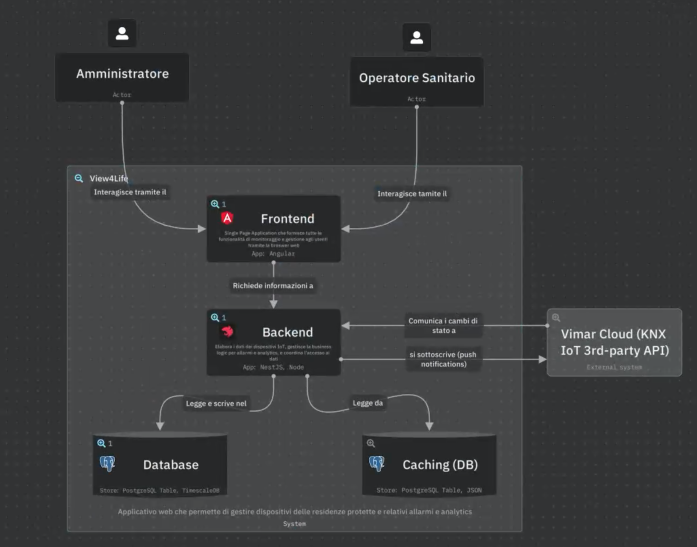
\includegraphics[
    width=\textwidth,
    height=0.8\textheight,
    keepaspectratio
  ]{Container-c4.png}
\end{frame}


\begin{frame}{Tecnologie scelte}
 \centering
  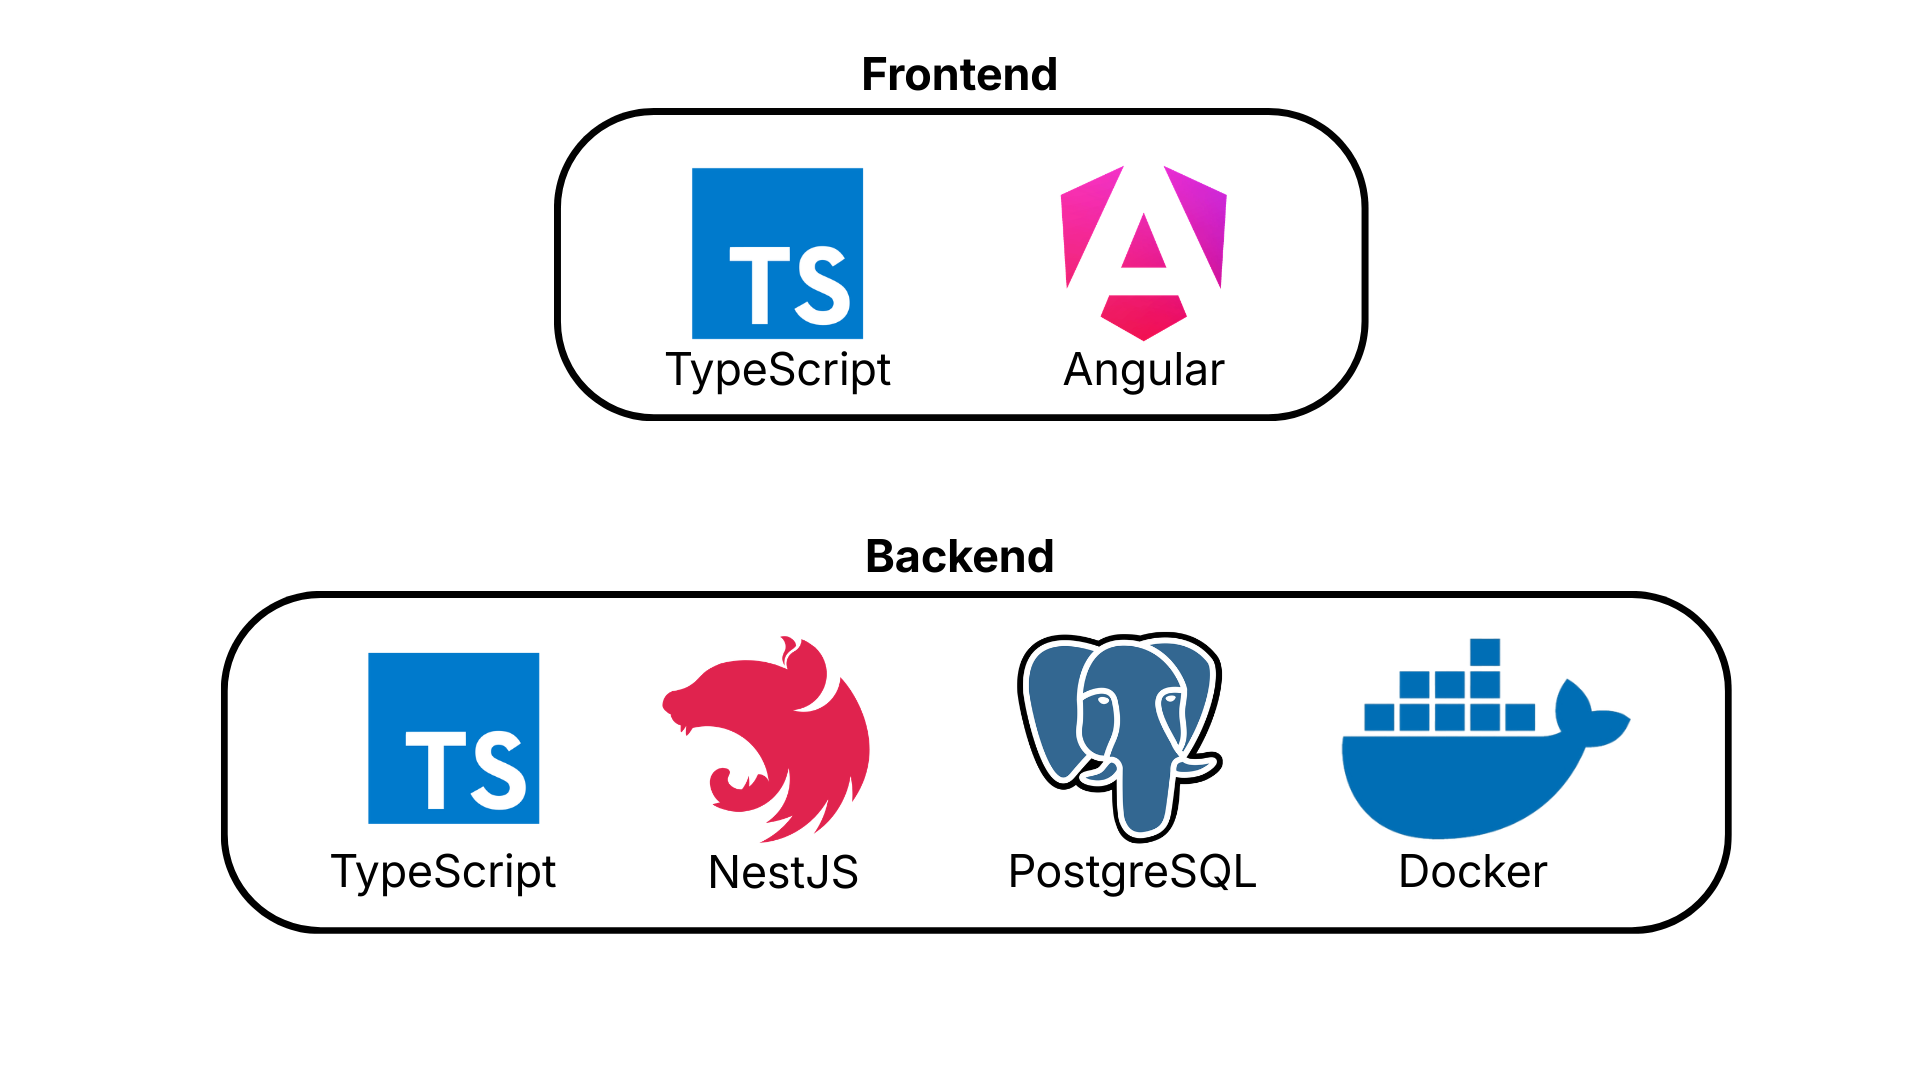
\includegraphics[
    width=\textwidth,
    height=\textheight,
    keepaspectratio
  ]{Tecnologie.png}
\end{frame}
 
\begin{frame}{Struttura Docker}
\end{frame}

\begin{frame}{Aspetti positivi del progetto}
Gli aspetti positivi riscontrati dal gruppo durante il progetto sono:
\begin{itemize}
    \item Sviluppo delle competenze di comunicazione e collaborazione 
          all'interno di un team strutturato.
    \item Acquisizione di nuove conoscenze tecniche legate 
          alle tecnologie adottate.
    \item Realizzazione di un prodotto con impatto concreto, 
          grazie alla collaborazione con un'azienda reale.
    \item Sperimentazione della metodologia Scrum per la gestione del progetto, 
          con organizzazione del lavoro in sprint.
    \item Esposizione a un flusso di lavoro professionale, 
          che include versionamento, documentazione e coordinamento del team.
\end{itemize}
\end{frame}

\begin{frame}{Aspetti negativi del progetto}
Gli aspetti negativi riscontrati dal gruppo durante il progetto sono:
\begin{itemize}
    \item Leggero disallineamento sui requisiti di progetto tra team e Proponente.
    \item Difficoltà nella definizione di previsioni corrette.
    \item Difficoltà nel rispetto delle scadenze.
    \item Sporadica mancanza di comunicazione, che ha comunque provocato rallentamenti.
    \item Carico di lavoro? (documentale?).
\end{itemize}
\end{frame}

\end{document}